\section{Frontend}

\subsection{Descrizione generale}

Il frontend dell'applicazione andrà a costituire il ruolo di \textit{View} nel pattern MVC. In particolare tale componente dell'applicazione è costituita da un sottosistema che implementa l'architettura \textit{Flux} proposta da \textit{Facebook}. Tale architettura si basa sul creare un sistema che abbia un \textit{data-flow} unidirezionale al fine di semplificare le interazioni tra le varie componenti e di assicurare che tra le componenti non esistano dipendenze circolari.
Nella progettazione secondo l'architettura \textit{Flux} si è seguito in particolare il principio che nessuna classe modifichi direttamente lo stato di un'altra ma che vengano create delle componenti che richiedono un'interazione delle \textit{Action} per comunicare con le altre parti del sistema.

\begin{figure}[h]
\centering
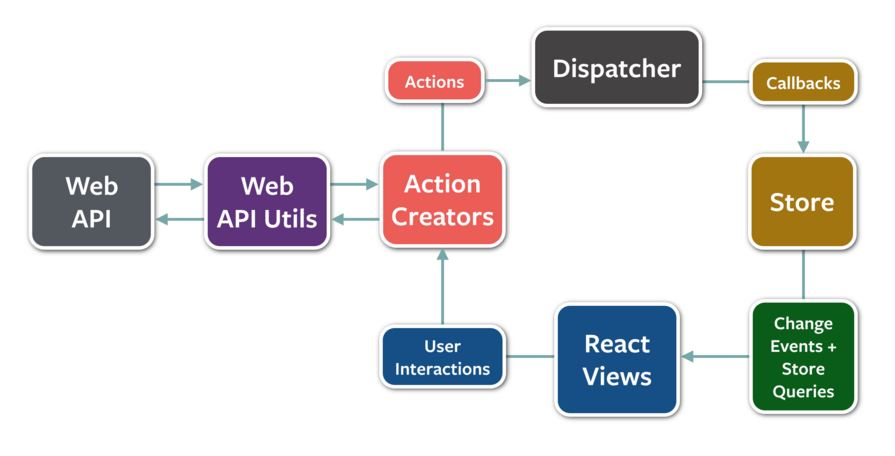
\includegraphics[width=0.8\textwidth]{res/sections/imgs/flux.jpg}
\caption{Diagramma dell'architettura Flux di Facebook}
\end{figure}
In un'architettura \textit{Flux} vengono distinti 4 componenti fondamentali:

\begin{itemize}
\item \textbf{Action}: Rappresenta un messaggio tra le componenti del sistema;
\item \textbf{Dispatcher}: funge da \textit{hub} centrale per le \textit{action} e si occupa di distribuirle al giusto \textit{store};
\item \textbf{Store}: contengono la logica applicativa del frontend e lo stato dei dati dall'ultimo \textit{update}. Si occupano di fornire i dati alle viste, quando queste li richiedono;
\item \textbf{View}: Sono la parte visiva dell'applicazione e, nel nostro caso, saranno costituite da componenti definite con React.
\end{itemize}

Dall'architettura sopra descritta sono stati individuati i seguenti package per il lato frontend di MaaS:

\begin{figure}[h]
\centering
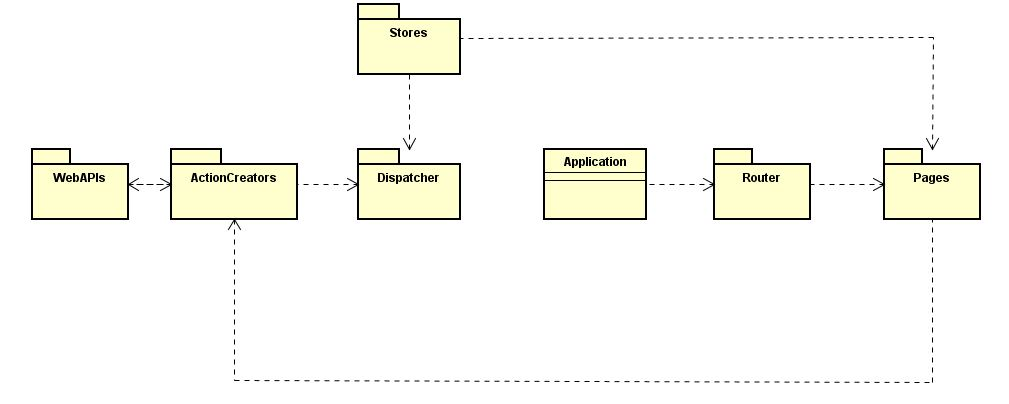
\includegraphics[width=0.8\textwidth]{res/sections/imgs/packages-diagram.jpg}
\caption{Diagramma dei package del frontend}
\end{figure}

\section{Descrizione dei package del frontend}
\subsection{WebAPIs}

\begin{figure}[h]
\centering
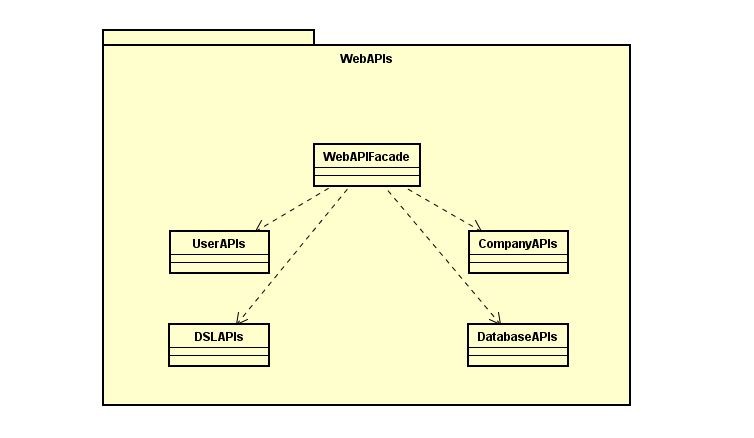
\includegraphics[width=0.8\textwidth]{res/sections/imgs/webapi-diagram.jpg}
\caption{Diagramma dei package del frontend}
\end{figure}

\paragraph*{Descrizione del package}
Il seguente package contiene tutte le classi che contengono i metodi per interagire con le API esposte dal server. 
\paragraph*{Classi contenute}
\begin{itemize}
\item \textbf{UserAPIs};
\item \textbf{CompanyAPIs};
\item \textbf{DSLAPIs};
\item \textbf{DatabaseAPIs};
\item \textbf{WebAPIFacade}.
\end{itemize}

\subsubsection{UserAPIs}
\paragraph*{Descrizione della classe}
Classe che espone tutti i metodi per interagire con le API del server che riguardano gli utenti.

\paragraph*{Utilizzo}
Viene utilizzata sia per il login sia per gestire le operazioni CRUD per le informazioni riguardanti gli utenti.

\paragraph*{Relazione con altre classi}
\begin{itemize}
\item ActionCreators::UserActionCreator
\end{itemize}

\subsubsection{CompanyAPIs}
\paragraph*{Descrizione della classe}
Classe che espone i metodi per interagire con le API esposte dal server che riguardano le Company.

\paragraph*{Utilizzo}
Contiene le operazioni CRUD per interagire con le informazioni riguardanti le company utilizzando le API esposte dal backend.

\paragraph*{Relazione con altre classi}
\begin{itemize}
\item ActionCreators::CompanyActionCreator
\end{itemize}

\subsubsection{DSLAPIs}
\paragraph*{Descrizione della classe}
Classe che espone i metodi per interagire con le API esposte dal server che riguardano le specifiche DSL.

\paragraph*{Utilizzo}
Viene utilizzata per lanciare le operazioni CRUD associate alle API esposte dal backend.

\paragraph*{Relazione con altre classi}
\begin{itemize}
\item ActionCreators::DSLActionCreator
\end{itemize}

\subsubsection{DatabaseAPIs}
\paragraph*{Descrizione della classe}
Classe per interagire con le API esposte dal server che riguardano i database delle Company.

\paragraph*{Utilizzo}
Viene utilizzata questa classe per lanciare le operazioni CRUD esposte dalle API del backend.

\paragraph*{Relazione con altre classi}
\begin{itemize}
\item ActionCreators::DatabaseAPIs
\end{itemize}

\subsubsection{WebAPIFacade}
\paragraph*{Descrizione della classe}
Classe che implementa il \textit{design pattern} \textit{Facade} al fine di creare un'interfaccia semplificata per il resto delle componenti per interagire con le API esposte dal backend.
\paragraph*{Utilizzo}
Questa classe viene utilizzata come interfaccia per il frontend per comunicare con le API esposte dal backend.
\paragraph*{Relazione con altre classi}
\begin{itemize}
\item webAPIs;
\item actionCreators.
\end{itemize} 

\subsection{ActionCreators}

\begin{figure}[h]
\centering
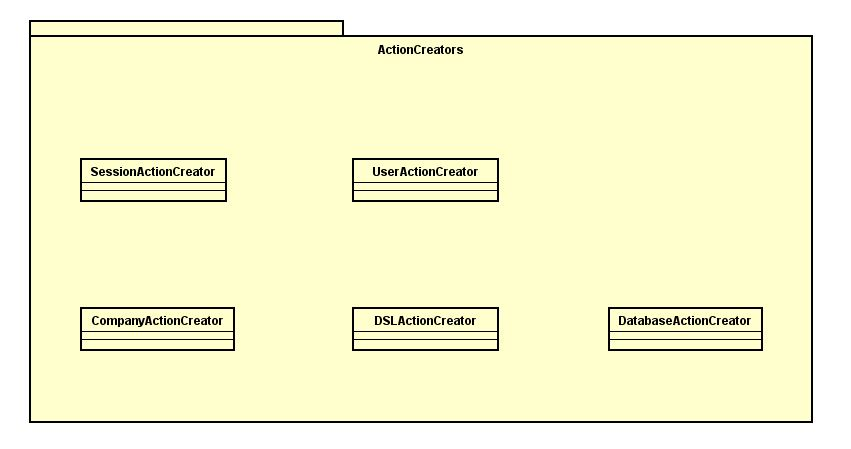
\includegraphics[width=0.8\textwidth]{res/sections/imgs/actioncreator-diagram.jpg}
\caption{Diagramma delle classi contenute in ActionCreators}
\end{figure}

\paragraph*{Descrizione del package}
Questo package contiene tutte le classi che si prestano come factory di Action. Le classi in questione mettono in relazione le webAPIs con il resto dell'applicazione, cioè vengono utilizzate per la richiesta delle funzionalità delle webAPIs per poi lanciare le Action relative alle risposte ricevute.

\paragraph*{Classi contenute}
\begin{itemize}
\item \textbf{SessionActionCreator};
\item \textbf{UserActionCreator};
\item \textbf{CompanyActionCreator};
\item \textbf{DSLActionCreator};
\item \textbf{DatabaseActionCreator}.
\end{itemize}

\subsubsection{SessionActionCreator}
\paragraph*{Descrizione della classe}
Classe che si occupa della gestione delle \textit{action} relative alla sessione corrente.

\paragraph*{Utilizzo}
Viene utilizzata per richiedere il login di un utente e per emanare le \textit{action} relative a login, sessione corrente e logout.

\paragraph*{Relazione con altre classi}
\begin{itemize}
\item Dispatcher;
\item Pages;
\item webAPIs::WebAPIFacade;
\item Stores::SessionStore.
\end{itemize}

\subsubsection{UserActionCreator}
\paragraph*{Descrizione della classe}
Classe che si occupa di creare e lanciare le \textit{action} relative agli utenti. Viene implementata tramite il \textit{design pattern} \textit{Factory}.
\paragraph*{Utilizzo}
Viene utilizzata per creare le \textit{action} relative agli utenti: la classe fornisce i metodi per utilizzare le \textit{webAPIs} contenute relative all'utente e restituisce le action che poi verrano reindirizzate a UserStore.

\paragraph*{Relazione con altre classi}
\begin{itemize}
\item Dispatcher;
\item Pages;
\item webAPIs::WebAPIFacade;
\item Stores::UserStore.
\end{itemize}

\subsubsection{CompanyActionCreator}
\paragraph*{Descrizione della classe}
Classe che si occupa dell'interazione dell'applicazione con CompanyAPIs e di lanciare \textit{Action} relative alle risposte ottenute da essa. Viene implementata tramite \textit{design pattern} \textit{Factory}.
\paragraph*{Utilizzo}
La classe viene utilizzata per creare le \textit{action} relative alle Company: sfrutta le \textit{webAPIs} dichiarate per interagire con il server e lancia le \textit{action} contenenti i dati ricevuti dalle API richieste.

\paragraph*{Relazione con altre classi}
\begin{itemize}
\item Dispatcher;
\item Pages;
\item Stores::CompanyStore;
\item webAPIs::WebAPIFacade.
\end{itemize}

\subsubsection{DSLActionCreator}
\paragraph*{Descrizione della classe}
Classe che si occupa di creare \textit{action} riguardanti le specifiche DSL.
\paragraph*{Utilizzo}
Tale classe viene utilizzata per sfruttare i metodi dichiarati dalle webAPIs per la richiesta delle API esposte dal server relative alle specifiche DSL. Dopo aver sfruttato l'API richiesta, la classe crea un'\textit{action} contenente i risultati ottenuti.

\paragraph*{Relazione con altre classi}
\begin{itemize}
\item Dispatcher;
\item Stores::DSLStore;
\item Pages;
\item webAPIs::WebAPIFacade.
\end{itemize}

\subsubsection{DatabaseActionCreator}
\paragraph*{Descrizione della classe}
Classe che si occupa di lanciare \textit{action} riguardanti le connessioni ai database di una Company.
\paragraph*{Utilizzo}
La classe viene utilizzata per richiamare i metodi definiti dalle \textit{webAPIs} relativi ai database delle Company e creare le action contenenti le risposte dai metodi chiamati.
\paragraph*{Relazione con altre classi}
\begin{itemize}
\item Dispatcher;
\item Pages;
\item Store::DatabaseStore;
\item webAPIs::WebAPIFacade.
\end{itemize}

\subsection{Dispatcher}
\paragraph*{Descrizione della classe}
Classe raffigurante il \textit{dispatcher} descritto nell'architettura Flux.
\paragraph*{Utilizzo}
Il dispatcher viene utilizzato come \textit{hub} centrale delle \textit{action} circolanti per l'applicazione. Esso deve fornire le informazioni per instradare le \textit{action} create dagli ActionCreators verso il giusto Store di destinazione
\paragraph*{Relazione con altre classi}
\begin{itemize}
\item Stores;
\item ActionCreators.
\end{itemize}


\subsection{Stores}

\begin{figure}[h]
\centering
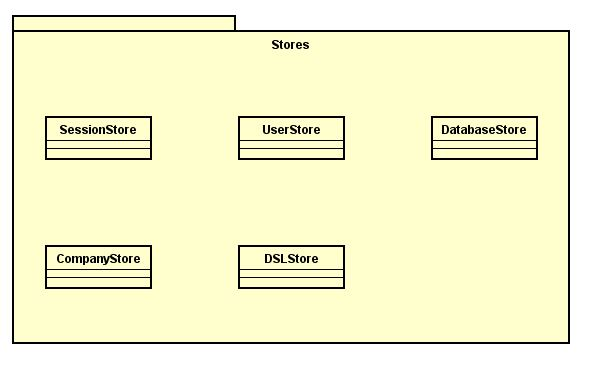
\includegraphics[width=0.8\textwidth]{res/sections/imgs/stores-diagram.jpg}
\caption{Diagramma delle classi per il package Stores}
\end{figure}

\paragraph*{Descrizione del package}
Il package in questione contiene le classi che implementano il concetto di Store presentato nell'architettura Flux. Ciascuno Store contiene dei dati omogenei tra loro e si occupa di fornirli alle pagine che ne necessitano.
\paragraph*{Classi contenute}
\begin{itemize}
\item \textbf{SessionStore};
\item \textbf{UserStore};
\item \textbf{DatabaseStore};
\item \textbf{CompanyStore};
\item \textbf{DSLStore}.
\end{itemize}

\subsubsection{SessionStore}
\paragraph*{Descrizione della classe}
Classe che contiene i dati relativi alla sessione corrente.
\paragraph*{Utilizzo}
Classe che viene utilizzata dall'applicazione per contenere e fornire i dati relativi alla sessione corrente. Si occupa di gestire le \textit{action} relative alla sessione e di conservarne i dati.
\paragraph*{Relazione con altre classi}
\begin{itemize}
\item Router;
\item Pages.
\end{itemize}

\subsubsection{UserStore}
\paragraph*{Descrizione della classe}
Classe che si occupa di contenere i dati relativi agli User.
\paragraph*{Utilizzo}
Questa classe viene utilizzata per mantenere i dati riguardanti gli utenti e di fornirli alle pagine che li richiedono.
\paragraph*{Relazione con altre classi}
\begin{itemize}
\item Pages;
\item Dispatcher.
\end{itemize}

\subsubsection{DatabaseStore}
\paragraph*{Descrizione della classe}
Classe che si occupa di contenere i dati relativi alle connessioni ai database definiti per le Company.
\paragraph*{Utilizzo}
Questa classe viene utilizzata per contenere i dati riguardanti le connessioni dei database definiti per le Company. Si occupa di ricevere dal dispatcher le \textit{action} relative a questi dati e di mantenere i dati riferiti.
\paragraph*{Relazione con altre classi}
\begin{itemize}
\item Pages;
\item Dispatcher.
\end{itemize}

\subsubsection{CompanyStore}
\paragraph*{Descrizione della classe}
Classe che si occupa di contenere i dati relativi alle Company.
\paragraph*{Utilizzo}
Questa classe viene utilizzata per ricevere le \textit{action} relative alle Company al fine di mantenere i dati relativi ad esse. Inoltre fornisce i metodi per fornire tali dati alle pagine che li richiedono
\paragraph*{Relazione con altre classi}
\begin{itemize}
\item Dispatcher;
\item Pages.
\end{itemize}

\subsubsection{DSLStore}
\paragraph*{Descrizione della classe}
Classe che si occupa di contenere i dati delle specifiche DSL
\paragraph*{Utilizzo}
Questa classe fornisce i metodi per ricevere le Action relative alle specifiche DSL e per mantenere i dati relativi ad esse. Fornisce inoltre i metodi per disporre quei dati per le pagine che li richiedono.
\paragraph*{Relazione con altre classi}
\begin{itemize}
\item Dispatcher;
\item Pages.
\end{itemize}


\subsection{Application}
\paragraph*{Descrizione della classe}
Questa è la classe principale del frontend: è la classe che richiama il Router e che inizializza il frontend.
\paragraph*{Utilizzo}
Viene utilizzata per inizializzare il frontend e per fornire le configurazioni necessarie al funzionamento per l'applicazione.

\subsection{Router}
\paragraph*{Descrizione della classe}
Questa classe è necessaria all'applicazione per determinare quale pagina mostrare.
\paragraph*{Utilizzo}
Viene istanziata nell'applicazione principale e determina le associazioni tra pagine e gli indirizzi URL per identificarle.

\subsection{Pages}
\paragraph*{Descrizione del package}
Questo package contiene tutte le pagine richiamate da Router. Ciascuna classe rappresenta una pagina definita come componente React e fornisce i metodi alla pagina per recuperare i dati da mostrare dagli store e i metodi per richiamare gli ActionCreators per la creazione di nuove Action.
